\section{Void-to-Absorber Problem}

\subsection{Purpose}

\subsection{Problem Description}

\subsection{Results}
\begin{figure}[h]
   \centering
   \begin{subfigure}{0.3\textwidth}
      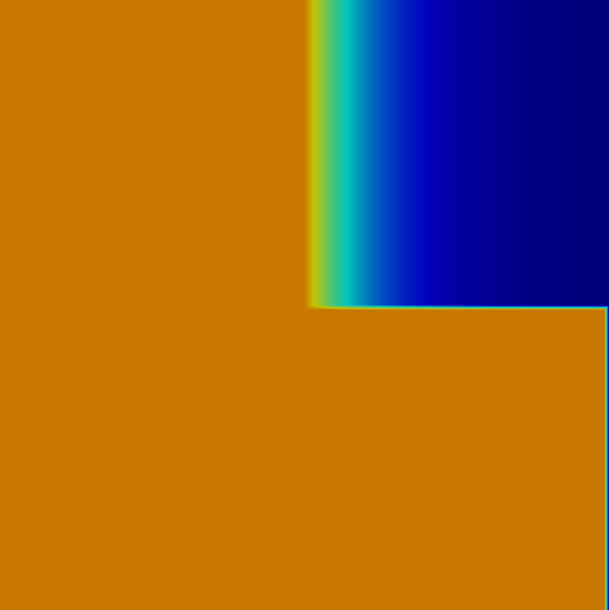
\includegraphics[width=\textwidth]{void_to_absorber/exact.png}
      \caption{Exact}
   \end{subfigure}
   \begin{subfigure}{0.3\textwidth}
      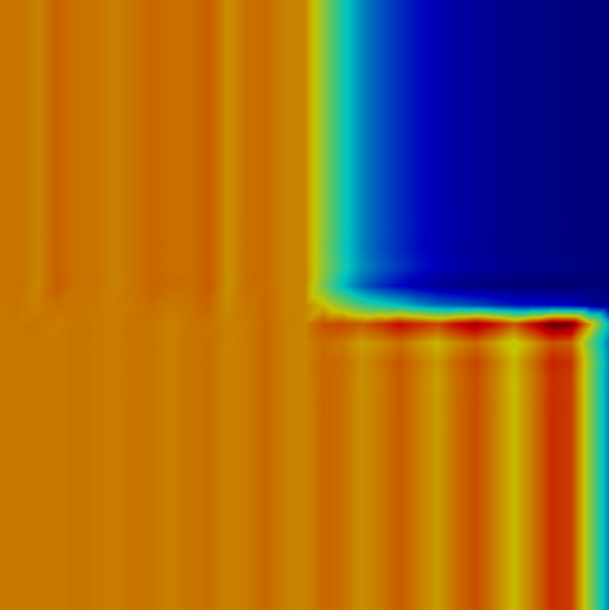
\includegraphics[width=\textwidth]{void_to_absorber/Gal.png}
      \caption{Galerkin}
   \end{subfigure}
   \begin{subfigure}{0.3\textwidth}
      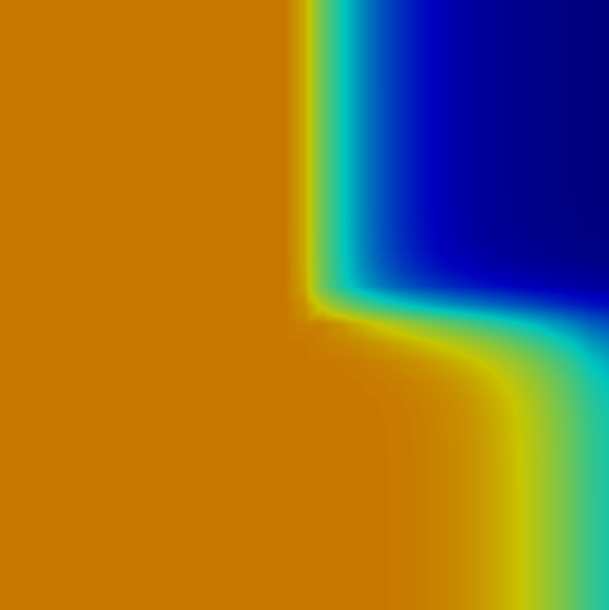
\includegraphics[width=\textwidth]{void_to_absorber/GalFCT.png}
      \caption{Galerkin with FCT}
   \end{subfigure}
   \begin{subfigure}{0.3\textwidth}
      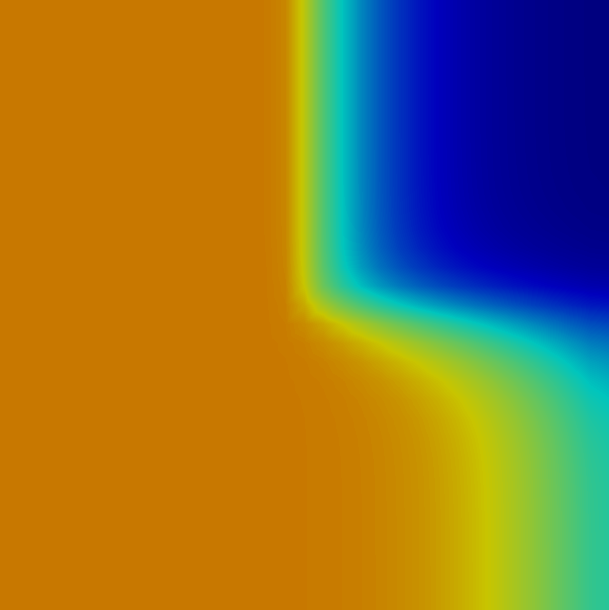
\includegraphics[width=\textwidth]{void_to_absorber/low.png}
      \caption{Low-order}
   \end{subfigure}
   \begin{subfigure}{0.3\textwidth}
      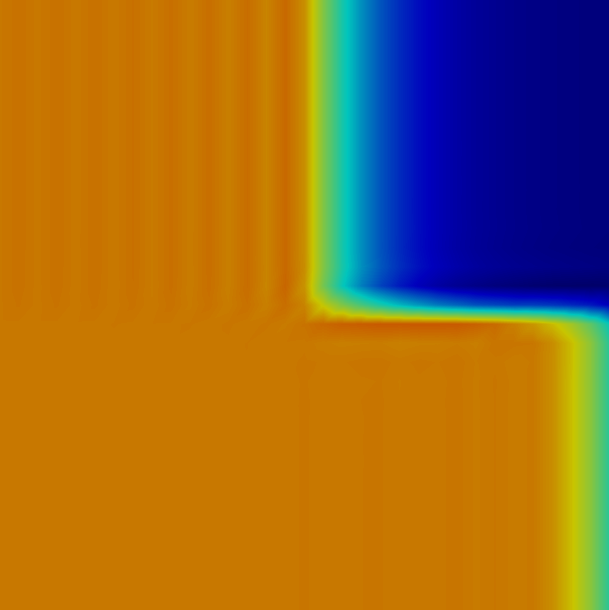
\includegraphics[width=\textwidth]{void_to_absorber/EV.png}
      \caption{Entropy Viscosity}
   \end{subfigure}
   \begin{subfigure}{0.3\textwidth}
      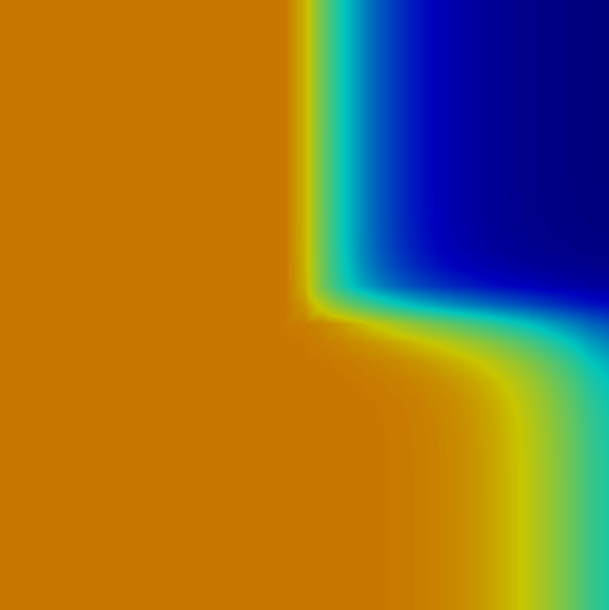
\includegraphics[width=\textwidth]{void_to_absorber/EVFCT.png}
      \caption{Entropy Viscosity with FCT}
   \end{subfigure}
   \caption{Comparison of Solutions}
\end{figure}

\subsection{Conclusion}

\subsection{Code and Version}

Version: eb86b4b97520531f7b13cee45d1514f9edfd2273
